Modellbildung der Strecke durch mathematische Beschreibungen der Wirkungszusammenh�nge zwischen den Systemgr��en, die f�r die Aufgabenstellung relevant sind.

Ein Modell ist eine aufgabenspezifische Vereinfachung der Realit�t. In der RT bew�hrte Modellierungsform:

\section{Darstellung der Strecke als Strukturbild (Blockschaltbild)}
\subsection{Beispiel: Permanten erregter Gleichstrommotor}
\begin{itemize}
	\item Ger�teschema: (siehe Beiblatt 4)
	\item Systemdarstellung:
\end{itemize}

\begin{center}
	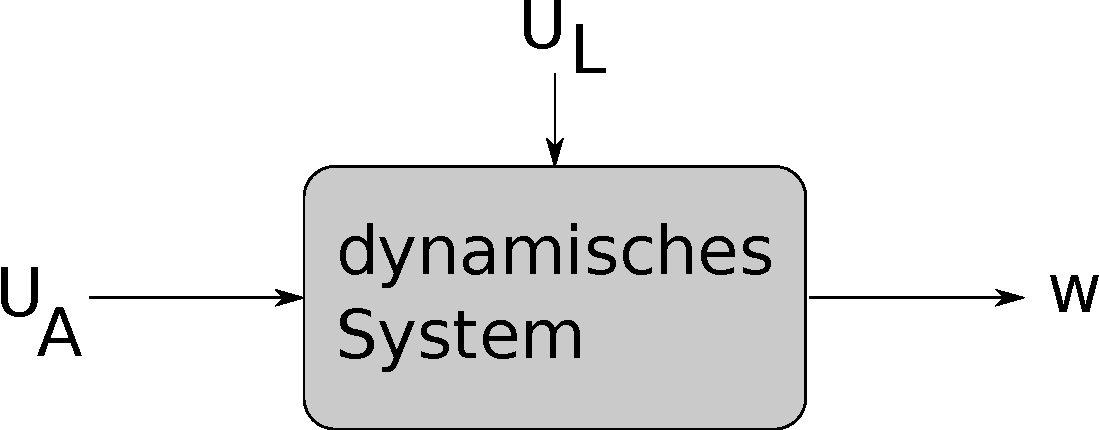
\includegraphics[width=200px]{graphics/gleichstrommotor.pdf}
\end{center}